\chapter{Countermeasures}
\section*{20 - Ottobre}
\section{Robust Programming}
Ideally it indicates a programming style focused on minimizing vulnerabilities and the impact of any vulnerability still exploitable.

\textbf{Robust programming} can be summarized with a few guidelines:
\begin{enumerate}
   \item \textit{Validate} program inputs aka input is evil
   \item \textit{Prevent} buffer overflow aka check sizes
   \item A robust implementation minimizes any \textit{information leaked outside} 
   e.g. module, object, function ...
   \note{
      \begin{itemize}
         \item Logical pointers rather than physical ones
         \item Validate any information that is exchanged
      \end{itemize}
   }
   \item Check values transmitted to other functions (egress filtering)
   \item Check returned results
\end{enumerate}
Besides, it is important to focus also on \textbf{interaction controls},
robustness must be enforced on both malicious and erroneous behaviour.

\subsection{Input validation}
Usually input validation is achieved with a form of \textit{default \textbf{deny}} by defining a legal input structure and discarding every input which doesn't satisfy it.
\note{In case of string this may be done through RegEx, max length, ...}

It is important that the checks to validate the input should be specified when the program is designed rather than after an attack;
besides a check should be designed in an simple and readable way,
to easily ensure its correctness.
Some examples of input which usually must be validated are:
\begin{itemize}
   \item Environment variables
   \item File names (blanks, .., /)
   \item Email addresses
   \item URL
   \item HTML headers/body
   \item Data
\end{itemize} 

Memory allocation and strings length is a crucial aspect:
only library functions with an explicit string length specified should be used\footnote{e.g. \lstinline|strncpy()| instead of \lstinline|strcpy()|},
and in general,
it is appropriate to
allocate only the memory actually needed by a data structure according to its sizeto avoid leaving
space to store dangerous values or inputs.\nl

Speaking of functions,
attention must be paid to a rigorous \textbf{interfaces definition} and to avoid making assumptions on relationships between input and output values of function;
in other words, if a function $A$ takes as input the value $x$ returned by $B$,
it must not be \textit{asserted} that $x$ is for sure a \textbf{valid} value,
$B$ should check the correctness of the input regardless of knowing how it was generated.

\subsection{CWE - Vulnerabilities Ranking}
\href{https://cwe.mitre.org/top25/archive/2023/2023_top25_list.html#tableView}{This article} by \textit{\textbf{CWE}} (\textit{Common Weaknesses Enumeration}) lists the most dangerous and frequent software weaknesses of 2023,
based on data provided by \textit{NIST}.

The scoring formula to calculate a ranked order of weaknesses
considers the \textbf{frequency} a CWE is the root cause of a vulnerability
with the \textbf{severity} of its exploitation. Both frequency and severity are
\textit{normalized} relative to the minimum and maximum values seen.
\textbf{Frequency} is obtained by counting weaknesses occurences in the \textit{National Vulnerabilities Database} (NVD),
while \textbf{severity} is the average computed on the Vulnerabilities score in the \textit{CVSS}\footnote{\textit{Common Vulnerabilities Scoring System}} a given weakness is mapped to.\\
The \textbf{final weakness score} is computed by multiplying frequency and severity scores.

\subsubsection{Biases and limitations}
There are two biases which CWE doesn't take into account,
which somehow negatively affect how valid CWE's scores are:
\begin{enumerate}
   \item \textbf{Metric bias}
   \begin{enumerate}
      \item 
      Indirect prioritization of implementation faults over design flaws
      \item 
      Prefers frequency over severity due to distributions of real-world
   \end{enumerate}
   \item \textbf{Data bias}
   \item \begin{enumerate}
      \item Only uses NVD data based on publicly-reported CVE Records
      \item Many CVEs do not have sufficient details to assign a CWE
      mapping, omitting them from ranking
      \item There may be an over-representation of certain programming
      languages, frameworks, or weakness-detection techniques
   \end{enumerate}
\end{enumerate} 

There also a few aspects which this scoring system cannot represent and should be taken care of.
First of all,
weaknesses that are rarely discovered will not receive a high score,
regardless of the consequence of an exploitation.
Weaknesses that begin with a root cause of a mistake leading to
other mistakes, create a chain relationship.
As we have seen, chains of mistakes/vulnerabilities/attacks are a key point in security,
but CWE's scoring system treats any $\langle V_1, V_2 \rangle \wedge V_1 \rightarrow V_2$ as if $V_1$ and $V_2$ were independent i.e. $V_1 \not\rightarrow V_2$.


\section{Firewall}
A \textbf{firewall} is a module to filter all the messages exchanged by \textit{two} networks with a distinct security level;
\textit{all and only} the messages travelling on the wires
connecting the two networks cross the firewall and therefore get filtered.
A firewall works correctly under the assumption that a network has been split (\textit{segmented}) into two \textbf{subnets}, 
and that it \textit{correctly implements} a security policy, which should \textit{\textbf{not}} define the policy by itself.
Firewalls are usually \textbf{classified} on the known and manageable \textbf{protocols} and on their \textbf{implementation}.

\subsection{Segmenting}
Firewalling goes along with \textbf{segmenting} a network,
which results in multiple subnets with different security levels whose interaction is determined by firewalls inbetween them.
This architecture increases \textbf{robustness} by preventing an attacker from having \textbf{initial access} on an entire system and from freely performing \textbf{lateral movements};
besides this architecture perfectly integrates with \textbf{honeypot} deception mechanisms.

\subsection{Classification}
Firewall may operate on different levels of the TCP/IP stack and in different ways:
\begin{itemize}
   \item Packet filtering firewall
   \item Circuit-level gateway
   \item Application-level gateway (aka \textit{Proxy Firewall}):
   firewall which recognizes application level protocols and can make assumptions on it
   \item Stateful inspection firewall
   \textit{Stateful} means that the firewall inspects also the contents of a communication and the properties related to the status of a connection.
   \item Next-generation firewall (NGFW)
\end{itemize} 

At level 3 (IP Packet Inspection) the firewall can check only the header of IP packets,
while at level 4 (circuit level firewall) ...\nl

TODO\nl

\subsection{Pros \& Cons analysis}

\subsubsection{Packet-filtering firewall}
\begin{paracol}{2}
   \vspace{\fill}
   \labelitemize{
      \textit{Pros}
   }{
      \begin{itemize}
         \color{darkgreen}
         \item A Single device can filter traffic for an entire network
         \item Extremely fast and efficient in scanning traffic
         \item Inexpensive
      \item Minimal effect on other resources, network performance and end-user experience
      \end{itemize}
   }
   \vspace{\fill}
   \switchcolumn
   \vspace{\fill}
   \labelitemize{
      \textit{Cons}
   }{
      \begin{itemize}
         \color{darkred}
         \item Since traffic filtering is entirely based on IP addresses and ports,
         it lacks broader context that informs other types of firewalls
         \item Doesn't check the payload and can be easily spoofed
         \item Not an ideal option for every network
         \item Access control lists can be difficult o set up and manage
      \end{itemize}
   }
   \vspace{\fill}
\end{paracol}

\subsubsection{Circuit-level gateway}
\begin{paracol}{2}
   \vspace{\fill}
   \labelitemize{
      \textit{Pros}
   }{
      \begin{itemize}
         \color{darkgreen}
         \item Only processes requested transactions; all other traffic is rejected
         \item Easy to set up and manage
         \item Low cost and minimal impact on end-user experience
      \end{itemize}
   }

   \vspace{\fill}
   \switchcolumn
   \vspace{\fill}
   \labelitemize{
      \textit{Cons}
   }{
      \begin{itemize}
         \color{darkred}
         \item No protection against data leakage from devices within the firewall that should be used in conjunction with other security technology
         \item No application layer monitoring
         \item Requires ongoing updates to keep rules current
      \end{itemize}
   }
   \vspace{\fill}
\end{paracol}


\subsubsection{Stateful inspection}
\begin{paracol}{2}
   \vspace{\fill}
   \labelitemize{
      \textit{Pros}
   }{
      \begin{itemize}
         \color{darkgreen}
         \item Monitors the entire session for the state of the connection, while also checking
         IP addresses and payloads for more thorough security only layer 4 information
         \item Offers a high degree of control over what content is let in or out of the network
         \item Does not need to open numerous ports to allow traffic in or out
         \item Delivers substantive logging capabilities
         \item Some defence against DOS
      \end{itemize}
   }
   \vspace{\fill}
   \switchcolumn
   \vspace{\fill}
   \labelitemize{
      \textit{Cons}
   }{
      \begin{itemize}
         \color{darkred}
         \item Resource-intensive and interferes with the speed of network communications
         \item More expensive than other firewall options
         \item No authentication capabilities to validate traffic sources aren't spoofed
      \end{itemize}
   }
   \vspace{\fill}
\end{paracol}
Most popular firewall as it acts as a gateway between computers and other assets
within the firewall and resources beyond the enterprise

\subsubsection{Application-level}
\begin{paracol}{2}
   \vspace{\fill}
   \labelitemize{
      \textit{Pros}
   }{
      \begin{itemize}
         \color{darkgreen}
         \item Examines all communications between outside sources and devices behind the
         firewall, checking not just address, port and TCP header information, but the
         content itself before it lets any traffic pass through the proxy. Layer 7 analysis
         \item Provides fine-grained security controls that can, for example, allow access to a
         website but restrict which pages on that site the user can open
         \item Protects user anonymity
   \end{itemize}
   }

   \vspace{\fill}
   \switchcolumn
   \vspace{\fill}
   \labelitemize{
      \textit{Cons}
   }{
      \begin{itemize}
         \color{darkred}
         \item Can inhibit network performance
         \item Costlier than some other firewall options
         \item Requires a high degree of effort to derive the maximum benefit from the
         gateway
         \item Doesn't work with all network protocols
      \end{itemize}
   }
   \vspace{\fill}
\end{paracol}
NGFWs are an essential safeguard for organizations in heavily
regulated industries, such as healthcare or finance

\subsubsection{NGFW}
\begin{paracol}{2}
   \vspace{\fill}
   \labelitemize{
      \textit{Pros}
   }{
      \begin{itemize}
         \color{darkgreen}
         \item Combines DPI with malware filtering and other controls to provide an
         optimal level of filtering. Considers also sender addresses
         \item Tracks all traffic from Layer 2 to the application layer for more
         accurate insights than other methods
         \item Can be automatically updated to provide current context
   \end{itemize}
   }
   \vspace{\fill}
   \switchcolumn
   \vspace{\fill}
   \labelitemize{
      \textit{Cons}
   }{
      \begin{itemize}
         \color{darkred}
         \item In order to derive the biggest benefit, organizations need to integrate
         NGFWs with other security systems, which can be a complex process
         \item Costlier than other firewall types
      \end{itemize}
   }
   \vspace{\fill}
\end{paracol}
NGFWs are an essential safeguard for organizations in heavily
regulated industries, such as healthcare or finance

\subsection*{Proxies}
\textbf{Proxies} protect clients from attacks from an external server,
while \textbf{reverse proxies} protect internal servers from attacks by external agents, 
besides they can also act as a load balancer.

\subsection{Wrapping Up}
\textbf{Stateful inspection} is the most common technology:
it works at the network layer and provides
dynamic packet filtering.
While packet filtering examines information in a
packet header, stateful inspection tracks each connection traversing any
firewall interface and confirms they are valid.
It is a system backed up by a state table that
tracks all sessions and inspects all packets passing through: 
if packets have
the properties the state table predicts, they can pass, otherwise they don't.
Clearly the state table changes
dynamically according to traffic flow.

\begin{figure}[ht]
   \centering
   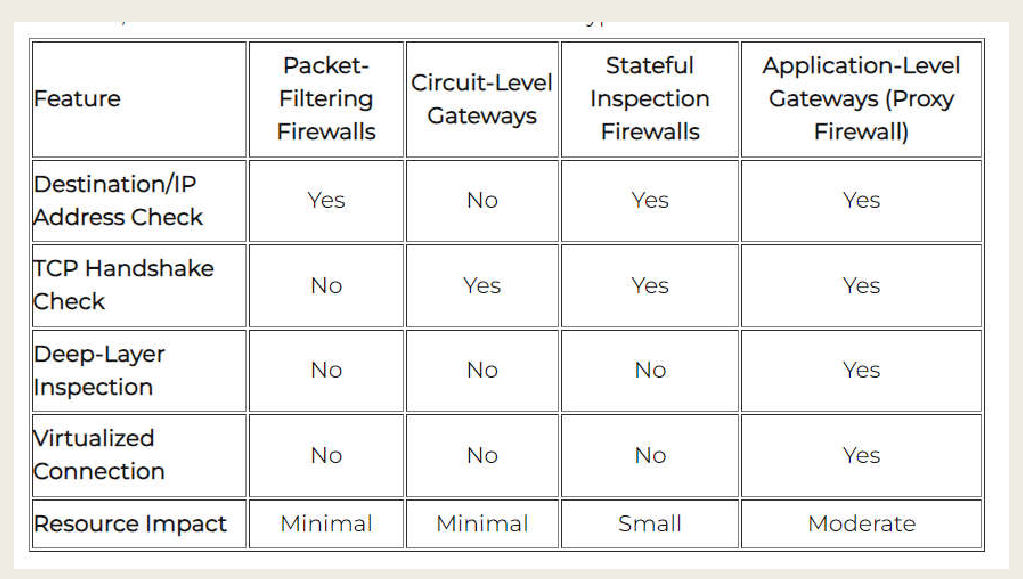
\includegraphics{images/firewall_comparison.png}
   \caption{Brief Firewall families comparison}
   \label{fig:firewall_comparison}
\end{figure}

\subsection{Takeaway guidelines}
These are the guidelines according to SNAS which indicate "suspicious" traffic \textbf{outgoing} from your network,
thus the network traffic which should be \textbf{egress-filtered}.
\begin{itemize}
   \item All traffic directed to IP addresses in your network(or that you manage)
   \item MS RPC (TCP/UDP 135), NetBIOS/IP (TCP/UDP 137-139), SMB/IP (TCP/445)
   \item Trivial File Transfer Protocol - TFTP (UDP/69)
   \item Syslog (UDP/514)
   \item Simple Network Management Protocol – SNMP (UDP 161-162)
   \item SMTP from all but your mail server
   \item Internet Relay Chat IRC (TCP 6660-6669)
   \item ICMP Echo/Reply
   \item ICMP Host Unreachable
\end{itemize}

\section{Segmentation}

A \textbf{segmented} network forces an attacker to adopt \textbf{pivoting},
which is attacking a host only to exploit it to route traffic to other nodes or subnets,
usually this is achieved with the aid of a \textbf{beacon} to remotely control the host.
Hence, in general, segmentation leads the attacker to implement \textit{more} attacks.

\begin{figure}[htbp]
   \centering
   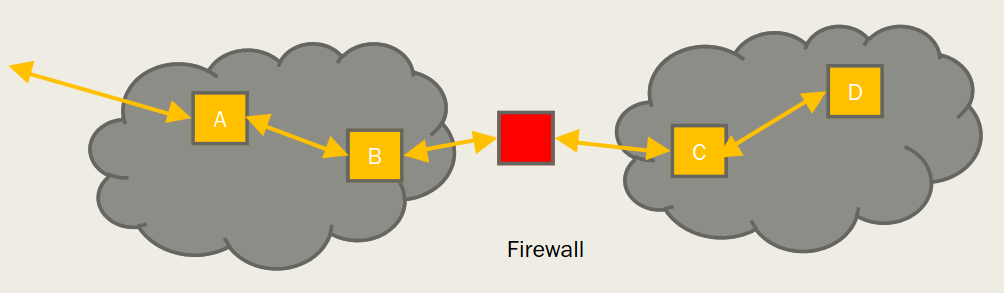
\includegraphics{images/pivoting.png}
   \caption{Segmented network and the need for Pivoting}
   \label{fig:pivoting}
\end{figure}

The attacker needs to perform pivoting to intrude in the network, thus they need to attack at least one host in left subnet and one in the right subnet;
otherwise they'd need to attack the firewall, but generally this is more costful in terms of effort and resources.

It is also possible to combine \textbf{firewalls} and \textbf{honeypots}.
They can be placed either in the internal network amongst other nodes or between the router and the global/outside network.

\subsubsection{Microsegmentation}

What about \textbf{cloud}-based computing?
The concept of firewalling still holds,
even for virtual networks,
but with a few adjustments.
\begin{figure}[htbp]
   \centering
   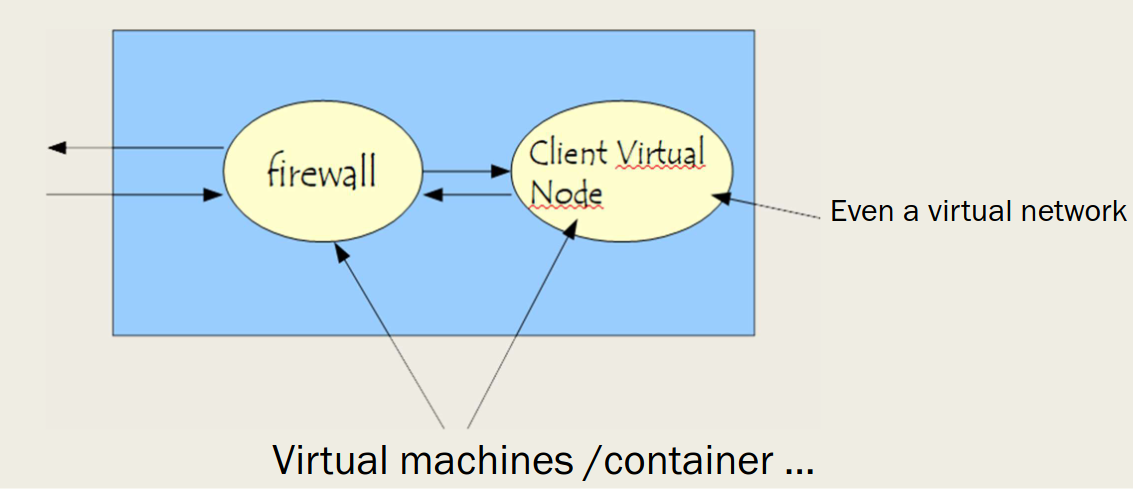
\includegraphics{images/firewall_cloud.png}
   \caption{Firewalling in cloud environments}
   \label{fig:firewall_cloud}
\end{figure}

\textbf{Microsegmentation} software with network virtualization technology is
used to create "zones" in cloud deployments.
These granular secure zones isolate \textit{workloads}, securing them individually with custom,
workload-specific policies.
This kind of granular security allows organizations to apply security controls to individual workloads and
applications, rather than having a single security policy for the entire server.

In this scenario, we can broadly define a \textbf{workload} as the resources and processes
needed to run an application. 
Hosts, virtual machines and containers are a few examples of workloads.
Since most modern enterprise systems are distrubuted among many cloud and local architectures, 
the goal of microsegmentation and zero trust is to overcome
\textbf{Perimeter Security} while protecting workloads.\nl

\textit{Perimeter security} makes up a significant part of most organizations’
network security controls.
Network security devices, such as network firewalls,
inspect “\textit{north-south}” (client $\rightarrow$ server) traffic that crosses the
security perimeter and block "bad" traffic.\\
Assets within the perimeter are instead implicitly trusted,
which means that “\textit{east-west}” (i.e. workload to workload) traffic may be allowed without inspection;
this is why \textbf{lateral movements} are usually hard to be identified.\\
Microsegmentation provides isolation and determines if two endpoints should access each other, hence
enforcing segmentation with least-privileged access reduces the scope of
lateral movements and might contains data breaches.
\begin{figure}[htbp]
   \centering
   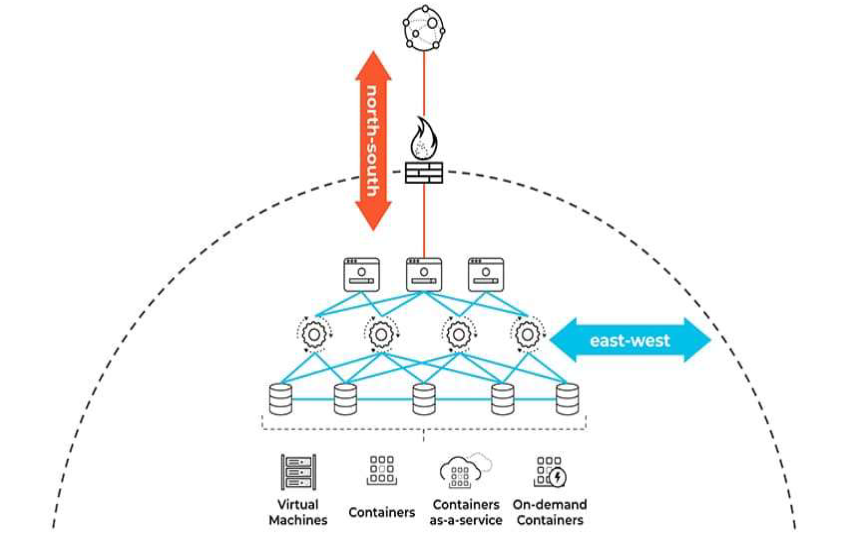
\includegraphics[width=0.4\textwidth]{images/microsegmentation_1.png}
   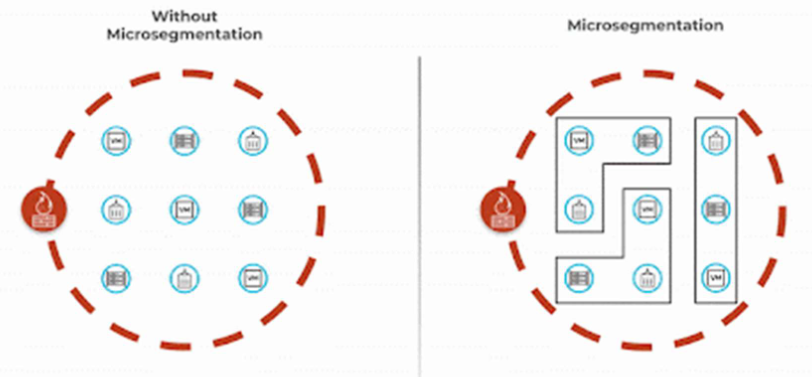
\includegraphics[width=0.4\textwidth]{images/microsegmentation_2.png}
   \caption{Microsegmentation example figures}
   \label{fig:microsegmentation}
\end{figure}

\subsubsection*{VLANs and Subnets}
VLANs virtually separate LANs into smaller networks,
they work like normal LANs but are logically or virtually separated instead of being
physically so.\\
Amongst reasons to use VLANs, the main one is to broadcast traffic.
VLANs give us all of the
benefits of physically separating our network, by doing it virtually without spending extra money on hardware and phyisical wiring management.

Subnets instead are networks inside a network or, in other words are smaller sections (subnetworks) of a larger network.
Basically, subnets are a logical partition of an IP network into several smaller
networks for making the network fast and efficient.

The key point is that VLAN are based on \textit{Layer-2} protocol, while subnet on \textit{Layer-3}.

\section{VPN}
A \textbf{Virtual Private Network} \textit{(VPN)} is an overlay network that emulates a secure connection on top of a public (\textit{unsecure}) network.
VPN connect local subnets that may even include just one machine.

\textbf{IPSEC} is an IPv4 extension to encrypt an authenticate information flow.
There are also other solutions to encrypt information also on different OSI layers, like PGP, HTTPs, SSL/TLS, ...
There are also network boards\footnote{FPGAs (?)} designed specifically to speed up IPSEC encryption/decryption.\\
IPSEC provides two possibile behaviours/protocols:
\begin{enumerate}
   \item \textbf{Authentication} Mode: auth header
   \item \textbf{Encapsulated Security Payload}: information encryption
\end{enumerate}
Besides, each of them can be used in two modes:
\begin{enumerate}
   \item \textbf{Transport} Mode: new fields are added to original packets.
   It is used to create a secure point-to-point connection between two nodes
   \item \textbf{Tunnel} Mode: IP packets become the payload of new IPSEC packets
   \note{This is the preferred and most popular way, since it may act transparently to internal nodes in a LAN,
   given that a host is delegated with the task of encrypting and decrypting}
\end{enumerate}


Each connection between nodes is protected using symmetric encryption while
the endpoints of the VPN may own a pair of public/private keys;
rhere is a protocol for the initial exchange that uses asymmetric encryption to
determine the shared key to create a secure connection between two nodes
that is protected through symmetric encryption.
In general symmetric encryption is better than asymmetric in terms of performance,
since it requires only basic operations like shifts and XOR.\nl

IPSEC defines 4 new protocols:
\begin{enumerate}
   \item \textbf{AH} \textit{Authentication header }- mutual authentication and message integrity
   \item \textbf{ESP} \textit{Encapsulating Security Payload }- it guarantees confidentiality by protecting all the content that is exchanged
   \item \textbf{IKE} \textit{Internet Key Exchange }- two partners reach a consensus on the key to be used to protect their communications and on how long such key is valid
   4 messages needed.
   \item \textbf{ISAKMP} \textit{Internet Security Association and Key Management Protocol }- to agree on the \textit{“Security Association (SA)”} to be established and on its attributes.\\
   6 messages needed, or 3 in case of \textit{ISAKMP-AGGRESSIVE}, which is usually preferred.
\end{enumerate}

The abovementioned \textbf{security association} (\textit{SA}) describes a direct connection with the
services associated with the traffic that crosses that connection;
it defines all the information needed to achieve a secure
communication.
The security services of a SA are implemented through either AH
or ESP, even if in principle the two protocols can be applied
simultaneously to the same connection this never happens in
practice.
Besides note that to defend a bidirectional communication two SAs are required,
one for each direction.\\
When negotiating on the SA the two nodes exchange a \textit{Security Parameters Index} \textit{SPI} used to lookup in a \textit{Security Associations Database SAD}.
\begin{figure}[htbp]
   \centering
   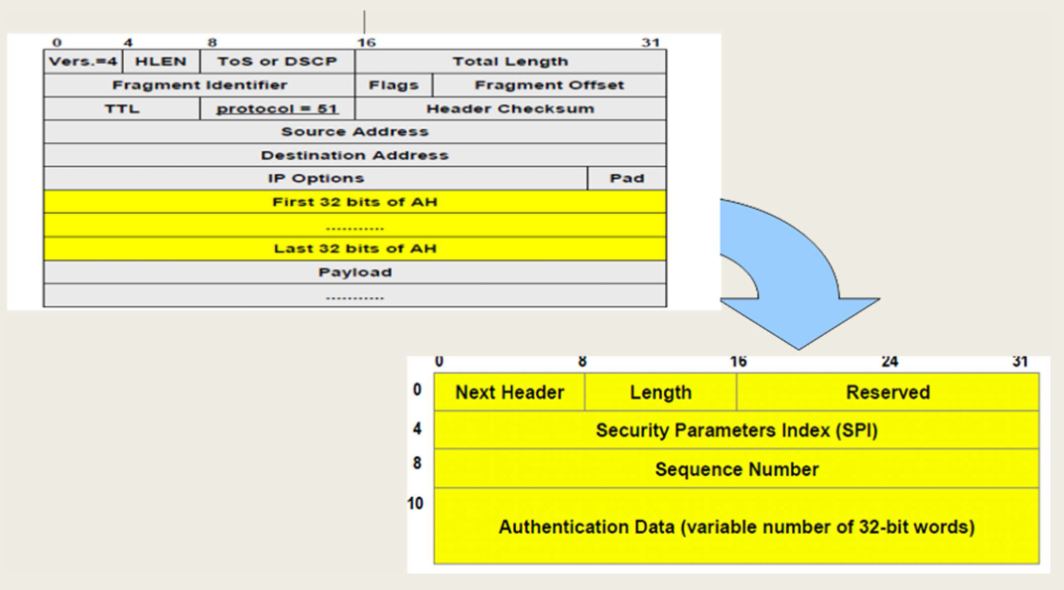
\includegraphics{images/IPSEC_ah.png}
   \caption{Authentication Mode header}
   \label{fig:IPSEC_ah}
\end{figure}
\begin{figure}[htbp]
   \centering
   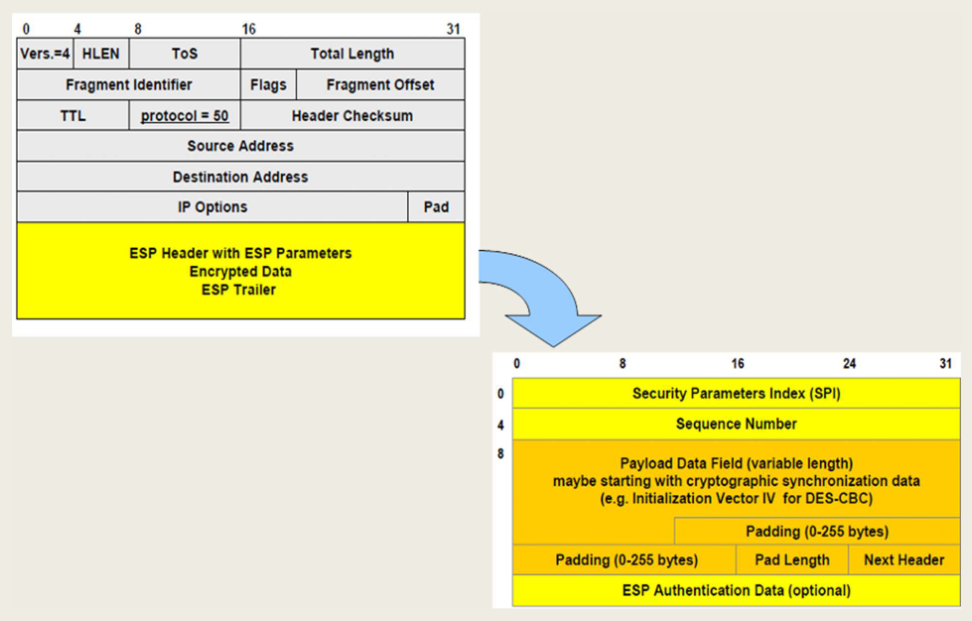
\includegraphics{images/IPSEC_esp.png}
   \caption{ESP mode}
   \label{fig:IPSEC_ah}
\end{figure}
